
\documentclass[12pt,a4paper,UTF8]{article}
\usepackage{ctex} % Chinese support
\usepackage{graphicx} % Insert images
\usepackage{listings} % Print source code
\usepackage[usenames,dvipsnames]{xcolor}
\usepackage{color} % Color support
\usepackage{float}
\usepackage{booktabs} % Professional table support
\usepackage{pdflscape} % Landscape pages support in PDF
\usepackage{hyperref} % Hypertext links support for cross-referencing
% \lstnewenvironment{cpp}{\lstset{language=cpp,
% 	basicstyle=\ttfamily\footnotesize,
% 	keywordstyle=\bfseries\color[rgb]{0, 0, 1},
% 	identifierstyle=\color[rgb]{0.5, 0.3, 0.1},
% 	stringstyle=\color[rgb]{0.6, 0.1, 0.1},
% 	commentstyle=\itshape\color[rgb]{0.05, 0.5, 0.05},
% 	backgroundcolor=\color[gray]{0.95},
% 	numbers=left,numbersep=5pt,numberstyle=\color[gray]{0.6},
% 	breaklines=true}}{}
\definecolor{mygreen}{rgb}{0,0.6,0}
\definecolor{mygray}{rgb}{0.5,0.5,0.5}
\definecolor{mymauve}{rgb}{0.58,0,0.82}
\lstset{
 backgroundcolor=\color{lightgray}, 
 basicstyle = \footnotesize,       
 breakatwhitespace = false,        
 breaklines = true,                 
 captionpos = b,                    
 commentstyle = \color{mygreen}\bfseries,
 extendedchars = false,             
 frame =shadowbox, 
 framerule=0.5pt,
 keepspaces=true,
 keywordstyle=\color{blue}\bfseries, % keyword style
 language = C++,                     % the language of code
 otherkeywords={string}, 
 numbers=left, 
 numbersep=5pt,
 numberstyle=\tiny\color{mygray},
 rulecolor=\color{black},         
 showspaces=false,  
 showstringspaces=false, 
 showtabs=false,    
 stepnumber=1,         
 stringstyle=\color{mymauve},        % string literal style
 tabsize=2,          
 title=\lstname                      
}

% Customize hyperref format (it's set to no special format here)
\hypersetup{hidelinks}

% Declare directories to search for graphics files for graphicx
\graphicspath{{figures/}{logo/}}


% Define source code style for listings
\lstdefinestyle{verilog}{
  language=Verilog,
  basicstyle=\ttfamily\footnotesize,
  keywordstyle=\bfseries\color[rgb]{0, 0, 1},
  identifierstyle=\color[rgb]{0.3, 0.2, 0},
  stringstyle=\color[rgb]{0.6, 0.1, 0.1},
  commentstyle=\itshape\color[rgb]{0.05, 0.5, 0.05},
  backgroundcolor=\color[gray]{0.98},
  numbers=left,
  numbersep=5pt,
  numberstyle=\color[gray]{0.6},
  breaklines=true
}

% Define source code style for listings
\lstdefinestyle{cpp-style}{
  language=C++,
  basicstyle=\ttfamily\footnotesize,
  keywordstyle=\bfseries\color[rgb]{0, 0, 1},
  identifierstyle=\color[rgb]{0.5, 0.3, 0.1},
  stringstyle=\color[rgb]{0.6, 0.1, 0.1},
  commentstyle=\itshape\color[rgb]{0.05, 0.5, 0.05},
  backgroundcolor=\color[gray]{0.95},
  numbers=left,
  numbersep=5pt,
  numberstyle=\color[gray]{0.6},
  breaklines=true
}

% Define new command for title page
\newcommand{\reporttitle}[2]{
  \LARGE\textsf{#1}\quad\underline{\makebox[12em]{#2}}
}
\newcommand{\reportinfo}[2]{
  \large\makebox[4em]{\textsf{#1}}\quad\underline{\makebox[18em]{#2}}
}
% The document begins here
\begin{document}
  \begin{titlepage}
    \centering
    
    
\includegraphics[height=144pt]{figure/picture.png}\\[48pt] % Change the school logo here (See the logo/ directory) and adjust the height
    {\huge\textsf{植\ 物\ 大\ 战\ 僵\ 尸}}\\[48pt]
    \reporttitle{报告名称}{PVZ设计}\\[72pt]

    \reportinfo{课程名称}{高级程序设计}\\[8pt]
    \reportinfo{学生姓名}{时欣}\\[10pt]
    \reportinfo{学\hspace{\fill}号}{191220097}\\[8pt]
    \reportinfo{实验日期}{2021年4月3日}\\
        \vspace*{\fill}
  \end{titlepage}

  \tableofcontents
  \newpage

  \section{实验内容}
    实现一个基本版的植物大战僵尸,主要内容包括:
    \subsection{界面显示}
        \begin{enumerate}
          \item 3行7列的地块;
          \item 商店内容的显示;
          \item 计分表分值;
          \item 阳光拥有值的显示
          \item 光标显示————用于进入商店时,移动光标来选择购买的植物;确定购买后,移动光标来选择植物存放的地块,并在相应的地块显示植物;(除了种植的确认)如果确定
          后又取消("x"),则再次显示光标,重复以上步骤。
          \item 僵尸显示。
        \end{enumerate}

    \subsection{游戏主体}
        \begin{enumerate}
          \item 僵尸:普通僵尸;
          \item 植物:豌豆射手,向日葵;
          \item 攻击工具:子弹;
        \end{enumerate}

    \subsection{游戏逻辑}
        \begin{enumerate}
          \item 塔防逻辑:植物有其对应的生命值和攻击力(每秒对僵尸造成多少伤害),僵尸有其对应的生命值,攻击力(每秒对植物造成多少伤害)和速度(走到
          下一个地块需要多少秒)。\\
                当僵尸走到植物所在地块时可以对植物进行攻击;当植物的生命值减到0则植物死亡,从植物列表中移除,而僵尸可以走到下一个地
          块对其中的植物攻击。如果僵尸将最左侧地块的植物攻击致死,则游戏失败。\\
                豌豆射手的作用是每秒发射子弹,真正起作用的是子弹。子弹有其伤害值(一个子弹对僵尸造成多少伤害)和速度,当子弹与僵尸在同一个地块时,
          子弹对僵尸造成伤害,随后子弹消亡。当僵尸的生命值减到0则僵尸死亡。
          \item 购买逻辑:植物有其对应的阳光消耗值,选定购买以后,阳光拥有值扣除相应的数量。如果阳光拥有值不足,则无法购买,对用户给出提示。
          
        \end{enumerate}
    

\section{实验目标}
    实现较好的交互界面,完成游戏正确的逻辑,尽可能丰富植物和僵尸的种类。

\section{实验环境}
\begin{enumerate}
  \item 设计语言:c++
  \item 运行环境:Windows
  \item 设计环境:Visual Studio 2019
\end{enumerate}
  
\section{实验设计思路}
    运用c++语言,运用面向对象的思路设计。
    \begin{enumerate}
      \item 需要实现的各类间关系如下图
          \begin{figure}[H]
            \centering
          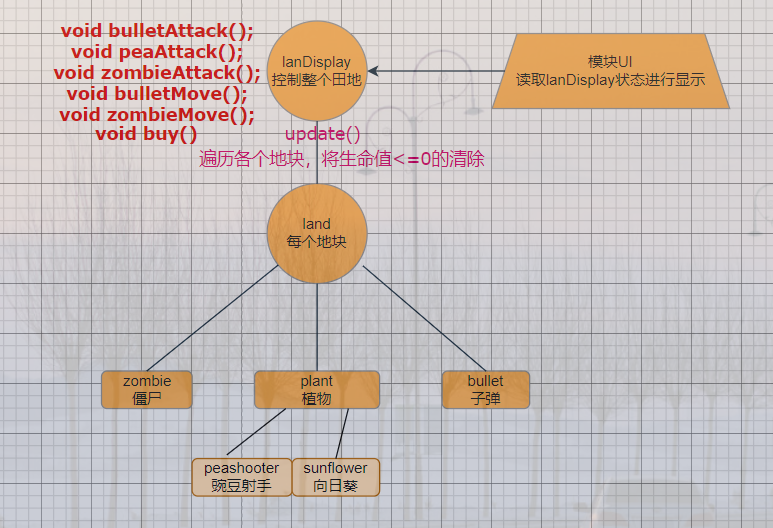
\includegraphics[width=0.9\textwidth]{figure/UMI.png}
          \caption{各类间关系}
          \end{figure}
        图中的各个图形标出的都是一个类(除了UI模块)。zombie,bullet,peashooter由land控制,而land由lanDisplay控制。(由于还没学到继承,所以plant下的植物以及zombie下的各种僵尸
        只是初步想法,实际实现的时候因为目前游戏主体还比较少,暂时还是用单独类实现的)。
    \item 设计思路\\
        如上图所示,lanDisplay类下有一个land类成员,而land类下有zombie,bullet,peashooter成员。采用类对象直接通信的机制。即lanDisplay类一旦发现zombie,bullet,peashooter的
        time==speed(在下面会有详细说明),则相当于这三个类对lanDisplay发送消息————我要移动了,或者我要攻击了。然后lanDisplay来控制,经过判断以后看能不能允许它们移动或者攻击。也就是
        能对地块状态进行改动的只有lanDisplay类,如果其它的类想要对地块状态进行改动,只能给lanDisplay发消息,通过lanDisplay来仲裁能否改动。\\
        而对于程序显示和定时刷新,我选择的是,每一轮攻击之后使用Sleep函数让程序休眠500ms,再继续,这样每一轮的输出都会停顿一下,以实现视觉上的动态变化效果。每一轮刷新,UI模块会
        读取lanDisplay的状态来输出。\\
        最后在main函数里面调用函数实行整个游戏的逻辑————用一个while循环,在游戏未失败的情况下,反复执行一轮一轮的攻击与移动。并且每当一段时间之后利用random随机选择一行产生僵尸,
        以及每当一段时间之后对系统阳光增加50.
    \end{enumerate}

\section{各个类的设计}
    \subsection{zombie类}
      \begin{figure}[H]
        \centering
      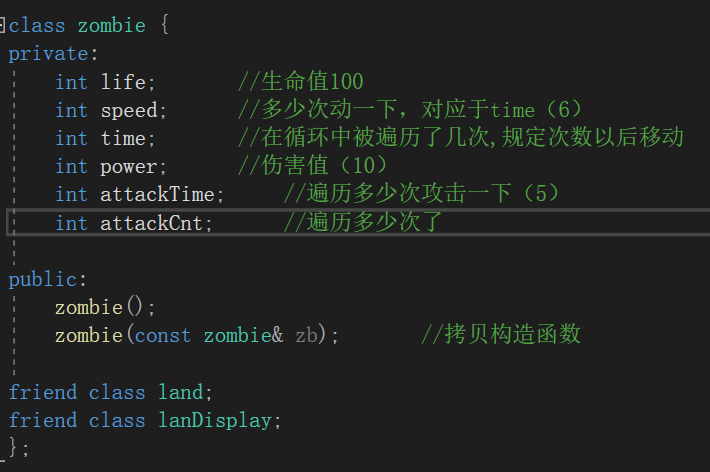
\includegraphics[width=0.7\textwidth]{figure/zombie.png}
      \caption{zombie类数据与操作}
    \end{figure}
      各个数据成员与成员函数的含义如注释所标。之所以要实现拷贝构造函数是因为,僵尸移动时需要带着它的状态(生命值等)走,也就是需要先在原先的
      地块删掉它, 然后在下一个地块新建一个和它一样的对象。
      如果被寒冰射手打中,那么减速时间持续五次遍历的时间,所以需要在每次遍历的时候对遍历次数的计数做额外处理。我没有另外写一个函数,而是直接放在僵尸的move里面了,也就是在判断
      完是否还活着以后,直接根据是否在减速的状态,就对其的计数做操作。

      僵尸的攻击比较复杂,采用虚函数和动态绑定,针对不同的情况给总控制类发出不同的返回值信号来显示自己需要干什么
      注意有道具的僵尸————撑杆僵尸和读报僵尸,在道具消失之后应该让其成为普通僵尸(而且生命值等状态需要延续,为此需要写非默认构造函数)
      而其中对于move来说
      \begin{enumerate}
        \item 撑杆僵尸: 它的move应该首先判断左边一格是否有植物并且此植物并非高坚果,如果true那么就向控制类发出信号1————表示请求跳过左侧植物;如果false,那么对遍历次数计数,
        和普通僵尸一样,到次数移动
        \item 投石僵尸:它的move需要判断石头有没有扔完石头,如果扔完了又到了移动的时候,那么就往左走。如果没有扔完但是左边没有任何植物,那么它也会往左走。
        \item 读报僵尸:它的move和普通僵尸一样,但是需要注意,给它变成普通僵尸的时候要增加移动速度,此处也需要通过非默认构造函数进行设置
        \item 路障僵尸和小丑僵尸:move和普通僵尸一样
      \end{enumerate}
      其中对于attack来说
      \begin{enumerate}
        \item 撑杆僵尸:它的attack是和普通僵尸一样(其实只有在面对高坚果的时候有效)
        \item 投石僵尸:它的attack是首先需要判断还有没有石头。如果有,那么到扔石头的时候,就告诉控制类要攻击植物了(从它的位置开始往左遍历,攻击最近的僵尸)。如果没有,就和普通僵尸
        一样,当前地块上有植物的话就让植物死亡
        \item 读报僵尸和路障僵尸:和普通僵尸一样
        \item 小丑僵尸:首先会有一个概率得出它要不要爆炸,如果不爆炸就和普通僵尸一样。如果爆炸就将周围3*3的植物都生命值置零。
      \end{enumerate}


    \subsection{peashooter类}
      \begin{figure}[H]
        \centering
      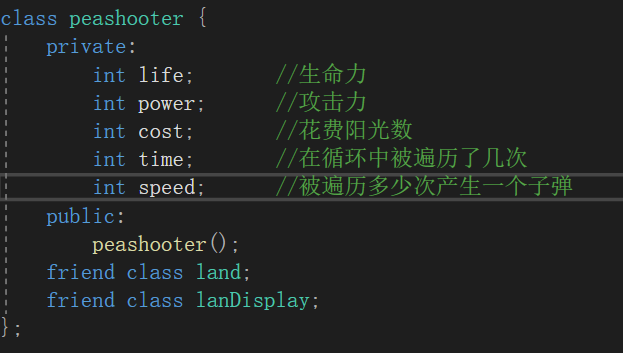
\includegraphics[width=0.65\textwidth]{figure/pea.png}
      \caption{peashooter类数据与操作}
      \end{figure}
      各个数据成员与成员函数的含义如注释所标。这个类比较简单,只需要实现默认构造函数即可。

    \subsection{bullet类}
    \begin{figure}[H]
      \centering
    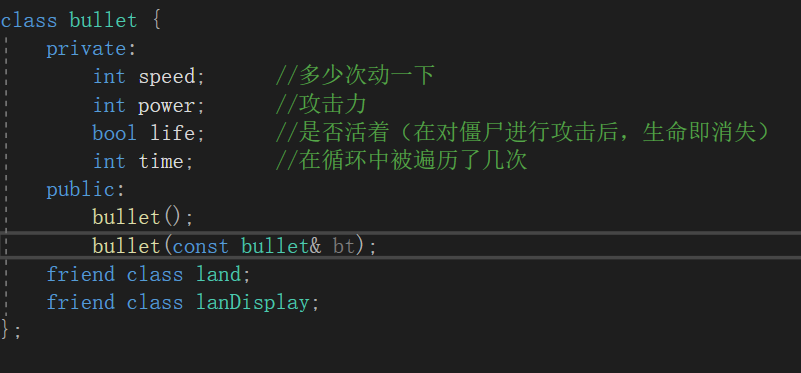
\includegraphics[width=0.8\textwidth]{figure/bullet.png}
    \caption{bullet类数据与操作}
    \end{figure}
    各个数据成员与成员函数的含义如注释所标。比较简单,不再赘述。

    \subsection{land类}
      \begin{figure}[H]
        \centering
      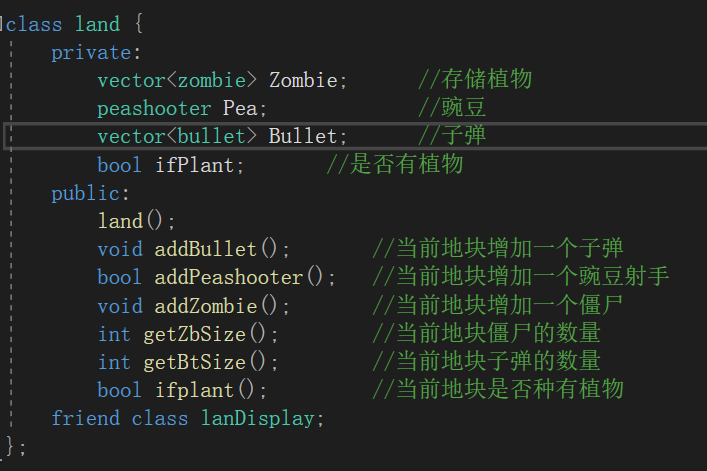
\includegraphics[width=0.7\textwidth]{figure/land.png}
      \caption{land类数据与操作}
      \end{figure}
      各个数据成员与成员函数的含义如注释所标。每一个land类的对象都是一块地块,各自管理各自的有关植物、僵尸和子弹的状态。

    \subsection{lanDisplay类}
    \begin{figure}[H]
      \centering
    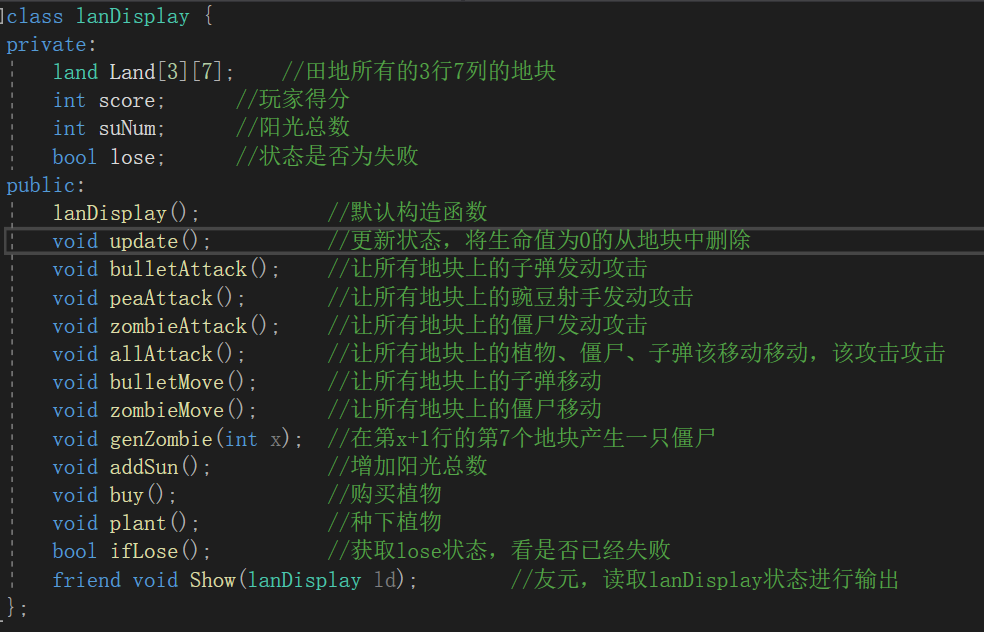
\includegraphics[width=0.7\textwidth]{figure/lanDis.png}
    \end{figure}
    \begin{enumerate}
      \item 各个数据成员与成员函数的含义如注释所标。lanDisplay类作为整个设计的核心控制类在本程序中占有极其重要的地位。
      \item 可以看到lanDisplay类中有数据成员land Land[3][7],即将所有地块以二维数组的形式进行组织,各个地块中又存储着属于自己的有关植物、僵尸和子弹的状态。
      \item 而lanDisplay类是land、植物、僵尸和子弹类的友元,因此通过lanDisplay类可以对地块的各种状态进行改动,从而实现对于地块中各个游戏主题的移动和攻击逻辑进行控制。
      \item lanDisplay类中的成员函数bulletAttack();是通过对于Land[3][7]中的每一个地块中的bullet成员进行遍历来实现的。回顾bullet类,它的数据成员有
      \lstinputlisting[style=verilog]{bullet.h}
      每一次遍历,如果发现子弹所在地块有僵尸,则僵尸被扣除子弹攻击一次会产生的伤害值,然后将子弹的生命值置零。
      \item peaAttack();也是通过对于Land[3][7]中的每一个地块中的bullet成员进行遍历来实现的。其实豌豆射手本身是不能对僵尸发动攻击的,因此它的攻击其实就是定时产生子弹。
      每一次遍历,如果发现time的值已经和speed的值相等则令豌豆射手产生子弹,否则time的值加一————以此来模拟豌豆射手的定时发射子弹。
      \item zombieAttack();是通过对于Land[3][7]中的每一个地块中的zombie成员进行遍历来实现的。攻击逻辑为:在当前地块有僵尸且其生命值大于0,并且当前地块有植物且其生命值大于0的情况下,
      如果僵尸的attackCnt的值已经和attackTime的值相等,则僵尸可以对植物发动攻击,对应的植物扣除相应的生命值。否则attackCnt的值加1————以此来实现僵尸对植物的定时攻击。
      \item bulletMove()是通过对于Land[3][7]中的每一个地块中的bullet成员进行遍历来实现的。如果当前地块没有僵尸,且子弹已经到了其该移动的时候————time==speed,则在下一个地块新建
      一个bullet,把当前地块的bullet删除,然后把time置零。如果还没到移动的时候,time的值加一。\\
      当然,如果已经在最后一个地块了,那么直接将其删除即可。当然,如果当前地块有僵尸,那么它暂时不能移动,因为接下来它需要对僵尸进行攻击。
      \item zombieMove()是通过对于Land[3][7]中的每一个地块中的zombie成员进行遍历来实现的。如果当前地块没有植物(ifPlant == 0),并且僵尸已经到了其移动的时候(time == speed),
      那么将当前地块的僵尸拷贝到下一个地块,将当前地块的僵尸删除。如果还没到移动的时候,那么将time的值增加一。\\
      需要注意,如果僵尸已经在最左边的地块而且也没有植物了,那么僵尸越过这个地块以后lanDisplay的lose状态将会被置为1,也就是说玩家失败。
    \end{enumerate}
    总的来说,lanDisplay类是通过与zombie,bullet,peashooter的通信来控制地块状态的,一旦发现它们的time==speed则相当于本类对lanDisplay发送消息————我要移动了,或者我要攻击了。
    而lanDisplay来判断,能不能允许它移动或者攻击。
    \begin{enumerate}
      \item 而update函数则是对地块状态进行更新,主要是全部遍历,将生命值为0的游戏主体从地块中删除,发现有多少死亡的僵尸,则将总分加上相应的加分,并且根据lose状态判断玩家是否失败
      来决定是否游戏结束。
      \item buy函数和plant函数本来是想放在lanDisplay类外面,单独作为一个类并和lanDisplay类交互的。可是因为是直接对lanDisplay中的地块状态进行操作,所以干脆放在了一个类里面。
      通过查阅资料,我知道了如何获取键码。\\
      我是通过光标的停留位置来判断用户的选择的。用户可以通过按下wasd键等来移动光标位置,y和enter来确认选择,x来取消。对地块的状态改动,是发生在
      选择好植物并确认种植以后,一旦获取到相应的键码,则在对应的地块上增加用户选择的植物。(当然如果判断到键码但发现阳光总数不够,则不会对地块进行改动,而是在界面下方对用户进行提示。\\
      相关代码为
      \lstinputlisting[style=verilog]{mouse.cpp}
      先判断是否有按键按下,如果有,获取键码,根据键码做相应事件。从买到种植,如果中间没有取消工作,是一个顺序循环读取键码的过程,所以采用while循环。
    \end{enumerate}

  
    
\section{程序亮点}
\begin{enumerate}
  \item 选择用一个类实现总控制的方法,模仿各个进程给操作系统发信息请求资源调度等让操作系统仲裁决定的方式,让其它类都给lanDisplay类发送自己的状态,而lanDisplay类接收到信息以后
  做出判断和相应操作。
  \item UI和游戏逻辑分离,只读取lanDisplay状态进行输出,不做别的多余的动作
  \item 游戏有主界面,当前有两个选项,如下图
  \begin{figure}[H]
    \centering
  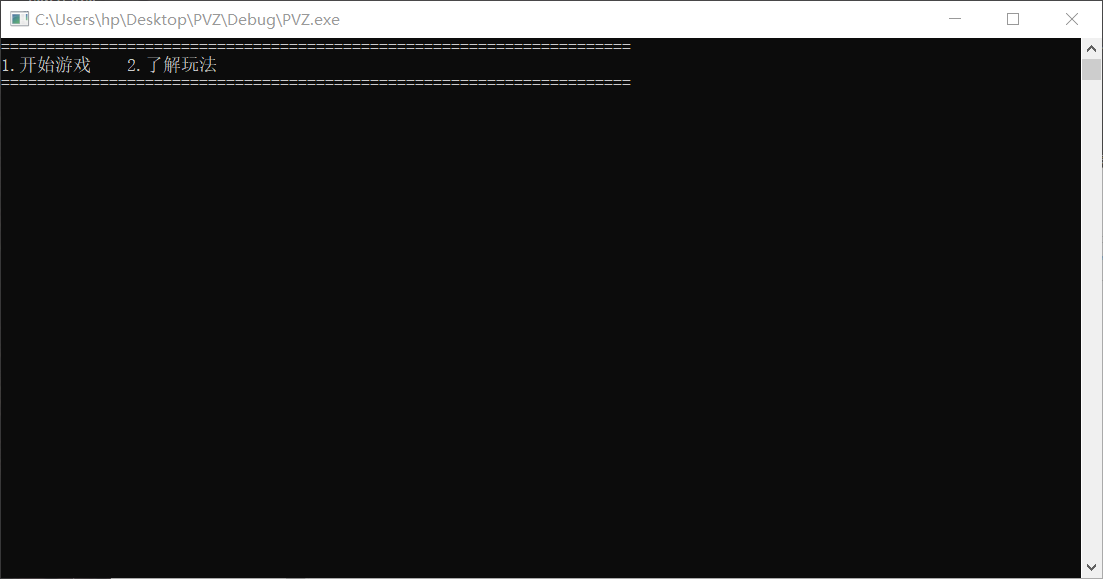
\includegraphics[width=0.7\textwidth]{figure/main.png}
  \caption{主界面}
  \end{figure}
  选择1则进入游戏界面,如下图
  \begin{figure}[H]
    \centering
  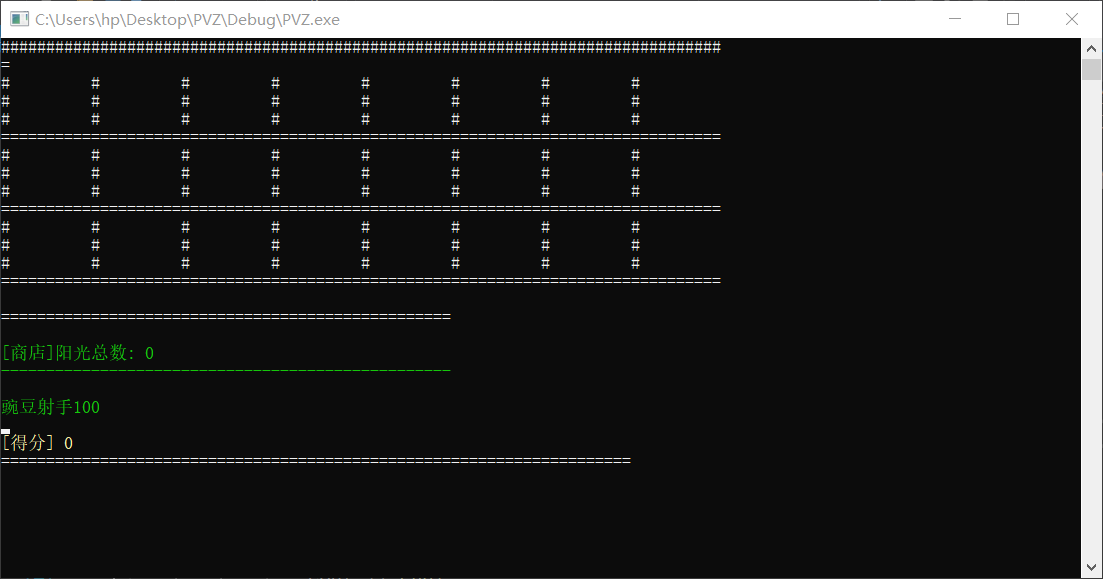
\includegraphics[width=0.7\textwidth]{figure/game.png}
  \caption{游戏界面}
\end{figure}
  选择2则进入游戏玩法说明,如下图
  \begin{figure}[H]
    \centering
  
\includegraphics[width=0.7\textwidth]{figure/rule.png}
  \caption{游戏规则}
  \end{figure}
  \item 对用户友好,如果阳光购买植物时不足会给出提示
  \begin{figure}[H]
    \centering
  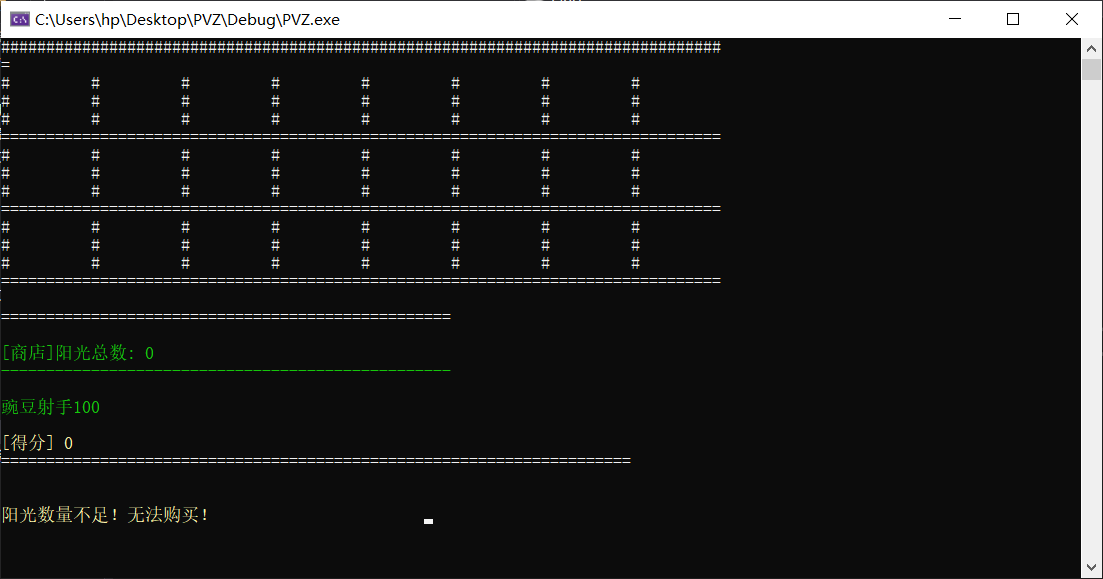
\includegraphics[width=0.7\textwidth]{figure/cout.png}\\
  \caption{提示如最后一行}
  \end{figure}
  不同的颜色更加醒目
  \begin{figure}[H]
    \centering
  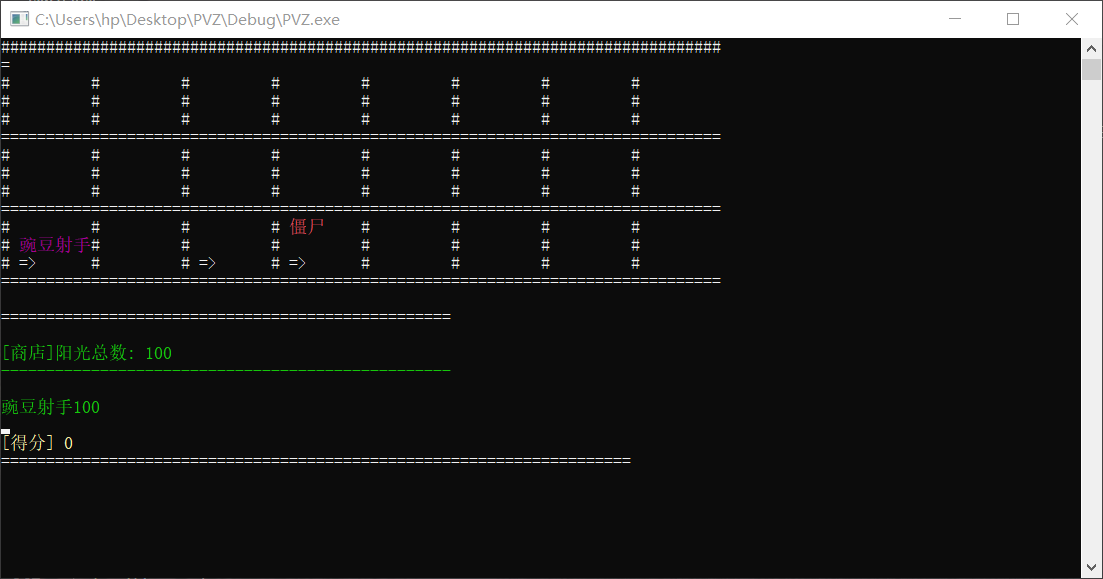
\includegraphics[width=0.7\textwidth]{figure/color.png}
  \caption{颜色展示}
  \end{figure}
  如果中途购买或种植时选择错误,可以按下“x”取消。
  如果用户游戏失败,会有一个持续1s的“游戏失败”提示,然后返回主界面,进行下一轮新的游戏。
  如果用户在已种植植物的地块上选择种植新的植物,会在游戏界面下方提示,并且可以重新选择。
\end{enumerate}
      
    
  
\section{玩法}
  \subsection{游戏开始界面}
  \begin{enumerate}
    \item 选择开始游戏则进入游戏界面
    \item 选择了解玩法,则显示游戏规则;按下enter则返回主界面。
  \end{enumerate}
  
  \subsection{商店购买规则}
  \begin{enumerate}
      \item 玩家可以通过按下"b"来选择需要购买的植物,按下"b"后,商店中对应的植物下方会出现光标,玩家在光标出现在想买植物下方时按下"y"键即可获得出现在地块上的光标进行种植。如果选择了
      并不存在的植物则无效。按下“x”键可以取消购买。
      \item 当光标在地块中显示时,玩家可以通过按下"w""s""a""d"表示上下左右,来移动,当光标出现在想选择的地块内时,按下“enter”即可在对应地块种下相应植物。按下“enter”后无法取消
      种植行为,而在这之前如果按下"x"可以回到商店选择界面。
      \item 商店会显示对应植物购买所需的阳光数,如果显示的阳光总数足够则可以进行购买;如果阳光不足,那么会在界面下方对用户进行提示
  \end{enumerate}

  \subsection{攻击规则}
  \begin{enumerate}
    \item 一共有3行7列地块。僵尸会随机出现在某一行的最右侧地块。玩家需购买植物来守卫自己的家(在游戏界面的最左边)。购买货币为阳光,由系统定时生成,总数显示在界面下方。
    \item 现有植物为豌豆射手,其功能为定时产生子弹。当子弹打到僵尸时,对僵尸造成定量伤害,随后这颗子弹被消耗。如果僵尸走到植物所在的地块,那么僵尸可以对植物进行攻击,直到植物被僵尸伤害至生命值
    为0,僵尸才可以走到下一个地块。
    \item 如果僵尸走到了最左边的地块(即家所在的最后一道防线),且地块上的植物被攻击致死,那么僵尸到达了“家”,玩家游戏失败。
  \end{enumerate}

  \subsection{计分规则说明}
    每打死一只僵尸,总分加五分。游戏为无尽模式,因此,只要僵尸并未攻击到“家”,则积分一直累计。

\subsection{总结与感想}
实验一开始的时候根本无从下手,感觉脑袋一团乱麻。后来自己一遍一遍的捋,总算大概有了个想法出来。只是当时是各个类自己管自己的攻击,于是写到这的时候发现不行,当每个类自己移动攻击的时候
是无法判断操作是否合理的。于是又重构,设计了一个总的控制类,让它来做所有会改变状态的操作。这样一来,思路清楚了很多。\\
主要遇到的bug其实是在输出对齐上。由于没有用宏,一些输出的偏移量感到不合适以后进行了改动,却在将输出位置转化为对应的地块坐标时出了错误。debug才发现没有全部改动好。于是改成了宏,
不得不说,在必要的地方用宏还是一个比较好的习惯。\\
而写完之后再回顾,发现还是并没有想象中那么难,要写的东西也并不多。主要是把逻辑理顺了,该注意的细节注意了就行。\\
后面学了继承应该是要对植物和僵尸的类进行重构的,否则一个一个类写过于繁杂重复。\\
希望如果有设计不合理的地方能够得到学长/学姐的建议(让我免于到最后时刻发现整个架构不行得要重构的绝望|・ω・`)),目前感觉好像还可以。


%\lstinputlisting[style=verilog]{md5_inout.v}

      
  \end{document}



